
\documentclass[a4paper,10pt,twoside,onecolumn]{report}

% Packages needed
\usepackage[T1]{fontenc}
\usepackage[utf8]{inputenc}
\usepackage{lmodern}         % Latin Modern fonts
\usepackage[english]{babel}
\usepackage{graphicx}
\usepackage{geometry}
\usepackage[]{tocbibind}     % Adding LoF, LoT and ToC itself to ToC
\usepackage{lipsum}          % Write "Lorem ipsum..." placeholder text
\usepackage{mathtools}
\usepackage{amssymb}
\usepackage{xcolor}
\usepackage{textcomp}        % Allow the use of upquote = true in \lstset
\usepackage{wrapfig}         % Wrap text around graphics (i.e. tip environment)
\usepackage{bookmark}
\usepackage{caption}
\usepackage{subcaption}

% Captions
\usepackage{caption}
\captionsetup
{
  margin = 30pt,
  skip = 10pt,
  justification = centering,
  labelfont = bf,
  textfont = it,
  font = small
}

% Custom colors
\definecolor{lightgray}{gray}{0.95}
\definecolor{orange}{rgb}{1,0.5,0}

% Code listings
\usepackage{listings}
\lstset
{
  basicstyle = \small\ttfamily,
  escapeinside = {<@}{@>},
  numbers = left,
  upquote = true,
%  frame = shadowbox,
%  frame = tRBl,
%  rulesepcolor = \color{lightgray},
  frame = single,
  columns = fullflexible,
  showstringspaces = false,
  tabsize = 8,
  keepspaces = true,
  rulecolor = \color{gray},
  commentstyle=\color{gray}\itshape,
  keywordstyle=\color{blue}\bfseries,
  backgroundcolor=\color{lightgray},
  stringstyle=\color{orange},
  numberstyle = \tiny,
  breaklines = true,
  postbreak = \raisebox{0ex}[0ex][0ex]{\ensuremath{\color{gray}\hookrightarrow\space}},
  caption = \lstname,
  literate = {á}{{\'a}}1 {é}{{\'e}}1 {í}{{\'i}}1 {ó}{{\'o}}1 {ú}{{\'u}}1
}

\usepackage{hyperref}
\hypersetup
{
  colorlinks = false,      % No link color
  linkbordercolor = gray,  % Gray link border
  urlbordercolor = gray,   % Gray URL border
  pdfborderstyle = {/S/U/W 0.5},
}

% Glossaries
\usepackage[acronym,toc]{glossaries}
\makeglossaries

\newacronym{adx}{ADX}{Average Directional Index}
\newacronym{ann}{ANN}{Artificial Neural Network}
\newacronym{ansi}{ANSI}{American National Standards Institute}
\newacronym{api}{API}{Application Programming Interface}
\newacronym{bb}{BB}{Bollinger Band}
\newacronym{bsd}{BSD}{Berkeley Software Distribution}
\newacronym{csv}{CSV}{Comma Separated Values}
\newacronym{ctf}{CTF}{C Tester Framework}
\newacronym{dd}{DD}{Dealing Desk}
\newacronym{ewt}{EWT}{Elliott Wave Theory}
\newacronym{gui}{GUI}{Graphical User Interface}
\newacronym{http}{HTTP}{Hypertext Transfer Protocol}
\newacronym{ipc}{IPC}{Inter-Process Communication}
\newacronym{jit}{JIT}{Just In Time}
\newacronym{ndd}{NDD}{No Dealing Desk}
\newacronym{ecn}{ECN}{Electronic Communication Network}
\newacronym{ema}{EMA}{Exponential Moving Average}
\newacronym{ide}{IDE}{Integrated Development Environment}
\newacronym{ip}{IP}{Internet Protocol}
\newacronym{lan}{LAN}{Local Area Network}
\newacronym{ma}{MA}{Moving Average}
\newacronym{macd}{MACD}{Moving Average Convergence/Divergence}
\newacronym{mpi}{MPI}{Message Passing Interface}
\newacronym{mt4}{MT4}{MetaTrader 4}
\newacronym{mt5}{MT5}{MetaTrader 5}
\newacronym{ohlc}{OHLC}{Open-High-Low-Close}
\newacronym{tohlcv}{TOHLCV}{Time-Open-High-Low-Close-Volume}
\newacronym{os}{OS}{Operating System}
\newacronym{oss}{OSS}{Open Source Software}
\newacronym{pas}{PAS}{Python Analysis Suite}
\newacronym{pca}{PCA}{Principal Components Analysis}
\newacronym{pgm}{PGM}{Pragmatic General Multicast}
\newacronym{pubsub}{PUB-SUB}{publisher-subscriber}
\newacronym{reqrep}{REQ-REP}{request-reply}
\newacronym{rhel}{RHEL}{Red Hat Enterprise Linux}
\newacronym{rsi}{RSI}{Relative Strength Index}
\newacronym{sma}{SMA}{Simple Moving Average}
\newacronym{ssh}{SSH}{Secure Shell}
\newacronym{stp}{STP}{Straight Through Processing}
\newacronym{svd}{SVD}{Singular Value Decomposition}
\newacronym{tcp}{TCP}{Transmission Control Protocol}
\newacronym{udp}{UDP}{User Datagram Protocol}
\newacronym{vcs}{VCS}{Version Control System}
\newacronym{nst}{NST}{New Strategy Tester}
\newacronym{nyse}{NYSE}{New York Stock Exchange}
\newacronym{wan}{WAN}{Wide Area Network}
\newacronym{zmq}{\O{}MQ}{ZeroMQ}



% Euro symbol
\usepackage[gen]{eurosym}
\DeclareUnicodeCharacter{20AC}{\euro{}}

% Graphics path configuration
\graphicspath
{
  {./images/}
% {/any/other/absolute/or/relative/path/}
}

\newenvironment{tip}
{
  \vspace{+10pt}
  \begin{it}
  \noindent
  \begin{minipage}{\linewidth}
  \rightskip=1cm
  \leftskip=1cm
  \setlength\intextsep{0pt}
  \begin{wrapfigure}[1]{l}[2cm]{0cm}
    \hspace{-1.5cm}
    
\includegraphics[width=1.5cm]{tip}
  \end{wrapfigure}
}
{
  {}
  \end{minipage}
  \end{it}
  \vspace{+10pt}
}

\newcommand{\cquote}[2]
{
  \begin{flushright}
    \begin{minipage}{0.6\linewidth}
      \raggedleft
      \small
      {
        ``\textit{#1}'' \\
        \vspace{5pt}
        \textit{\textbf{--- #2}}
      }
    \end{minipage}
  \end{flushright}
}

\begin{document}

% Set empty style (no numbering)
\pagestyle{empty}

% Title page
\begin{titlepage}
\begin{center}
	\ \\%
	\vspace{7.0cm}
	\LARGE{\textbf{My template}} \\
	\vspace{1.0cm}
	\Large{Miguel Sánchez de León Peque} \\
	\vspace{0.5cm}
	\large{\today}
\end{center}
\end{titlepage}



% Set plain style and roman page numbering
\pagestyle{plain}
\pagenumbering{roman}

% Table of contents, list of figures and list of tables
\tableofcontents
\listoffigures
\listoftables
\lstlistoflistings
\cleardoublepage

% Set headings style and arabic page numbering
\pagestyle{headings}
\pagenumbering{arabic}

\part{Styles}

\chapter{Basic styles}

\cquote{A quien no sabe a qué puerto se dirige, ¡mal viento lo lleve!}{Maxi Peque}

\section{Paragraphs, lists}

\subsection{Paragraphs}

Australia, Australia sí que es la hostia. ¿Tú sabes cuantos kilómetros cuadrados tiene Australia? Siete millones seiscientos y pico mil. Diez veces esto. ¿Y habitantes? Ni la mitad que aquí. Así que calcula. Calcula a lo que tocan por cabeza. Aquí no salimos a una mierda.

Porque te dan tu parte. Cuando te jubilas. Por una ley que hay. Dividen. Tantos Kilómetros de país los que sean, por tantas personas, tanto. No sé, ponle. Dos kilómetros cuadrados, tres, lo que toque. Y te lo dan. A cada uno su trozo, ¿Te imaginas? Toma, pum, lo tuyo. Para ti para siempre. Y tú haces ahí lo que te sale de los huevos.

\subsection{Lists}

The first formal definition of free software was published by FSF in February 1986. That definition, written by Richard Stallman, is still maintained today and states that software is free software if people who receive a copy of the software have the following four freedoms.

\begin{itemize}
  \item The freedom to run the program for any purpose.
  \item The freedom to study how the program works, and change it to make it do what you wish.
  \item The freedom to redistribute copies so you can help your neighbor.
  \item The freedom to improve the program, and release your improvements (and modified versions in general) to the public, so that the whole community benefits.
\end{itemize}

The first formal definition of free software was published by FSF in February 1986. That definition, written by Richard Stallman, is still maintained today and states that software is free software if people who receive a copy of the software have the following four freedoms.

\begin{enumerate}[label=(\alph*)]
  \item The freedom to run the program for any purpose.
  \item The freedom to study how the program works, and change it to make it do what you wish.
  \item The freedom to redistribute copies so you can help your neighbor.
  \item The freedom to improve the program, and release your improvements (and modified versions in general) to the public, so that the whole community benefits.
\end{enumerate}

The first formal definition of free software was published by FSF in February 1986. That definition, written by Richard Stallman, is still maintained today and states that software is free software if people who receive a copy of the software have the following four freedoms.

\begin{enumerate}
  \item The freedom to run the program for any purpose.
  \item The freedom to study how the program works, and change it to make it do what you wish.
  \item The freedom to redistribute copies so you can help your neighbor.
  \item The freedom to improve the program, and release your improvements (and modified versions in general) to the public, so that the whole community benefits.
\end{enumerate}

\lipsum[1]

\begin{description}
  \item[First item] \hfill \\
    \lipsum[2]
  \item[Second item] \hfill \\
    \lipsum[2]
\end{description}

\lipsum[1]

\begin{description}[style=multiline,leftmargin=1.0cm]
  \item[A0]
    A description list with short descriptions.
  \item[A1]
    A description list with short descriptions.
  \item[A2]
    A description list with short descriptions.
  \item[A3]
    A description list with short descriptions.
\end{description}

\lipsum

\section{Figures, tables and code}

\subsection{Figures}

\lipsum[1]

\begin{figure}[htbp]
  \centering
  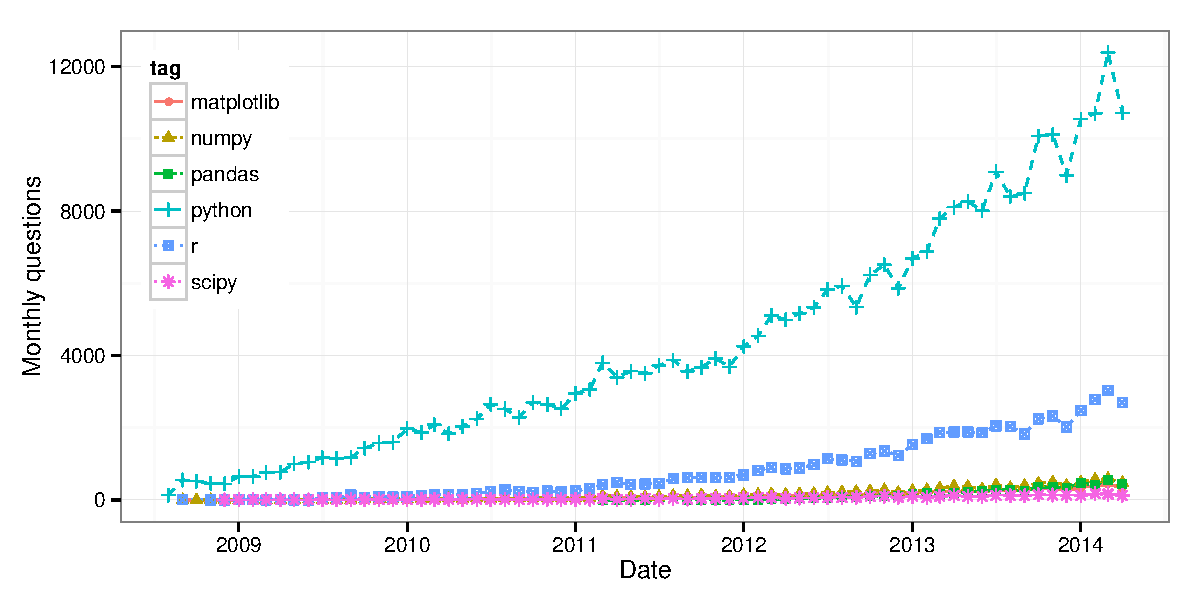
\includegraphics[width=0.9\textwidth]{stackexchange-r-vs-python}
  \caption{Comparison of the number of questions found in StackExchange for R, Python and some of the main Python scientific libraries in the last years.}
  \label{stackex-rpython}
\end{figure}

\lipsum[1]

\begin{figure}[htbp]
  \centering
  \begin{subfigure}[b]{0.3\textwidth}
    
\includegraphics[width=0.9\textwidth]{tip}
    \caption{Subfigure 0.}
    \label{resampling-00}
  \end{subfigure}
  \begin{subfigure}[b]{0.3\textwidth}
    
\includegraphics[width=0.9\textwidth]{tip}
    \caption{Subfigure 1.}
    \label{resampling-01}
  \end{subfigure}
  \begin{subfigure}[b]{0.3\textwidth}
    
\includegraphics[width=0.9\textwidth]{tip}
    \caption{Subfigure 2.}
    \label{resampling-02}
  \end{subfigure}
  \caption{Figure caption for all the four subfigures.}
  \label{resampling}
\end{figure}

\lipsum[1]

\subsection{Tables}

\lipsum[1]

\begin{table}[htbp]
  \caption{A table centering numbers at their decimal sepparator.}
  \label{table-example}
  \centering
  \begin{tabularx}{0.8\linewidth}{@{}LSS@{}}
    \toprule[1.5pt]\toprule
    & \multicolumn{2}{c}{\textbf{Count}} \\
    \cmidrule(r){2-3}
    \textbf{Module} & \textbf{Type 0} & \textbf{Type 1} \\
    \midrule
     Item 0 & 15.0 & 200.02 \\ Item 1 & 2.04 & 20.4 \\ Item 2 & 158 & 1308.1 \\
    \midrule
    \textbf{All} & 175.04 & 1528.52 \\
    \bottomrule\bottomrule[1.5pt]
  \end{tabularx}
\end{table}

\lipsum[1]

\begin{table}[htbp]
  \caption{Another table for goals.}
  \label{another-table-example}
  \centering
  \begin{tabularx}{0.4\linewidth}{@{}Lc@{}}
    \toprule[1.5pt]\toprule
    \textbf{Goal} & \textbf{Achieved}\\
    \midrule
    Goal 0 & \checkmark \\
    Goal 1 & \checkmark \\
    Goal 2 & \checkmark \\
    \bottomrule\bottomrule[1.5pt]
  \end{tabularx}
\end{table}

\subsection{Code}

\lipsum[1]

\begin{lstlisting}[caption=Getting data about Python and R questions in StackExchange, label=stackexchange-r-python, language=SQL]
SELECT *, count(*) AS count FROM (
	SELECT DATEADD(MONTH, DATEDIFF(MONTH, 0, CreationDate), 0) AS [month],
	       t.TagName AS [tag]
	FROM Posts p
		JOIN PostTags pt ON pt.PostId = p.Id
		JOIN Tags t ON t.Id = pt.TagId
	WHERE t.tagName IN ('python', 'r', 'scipy', 'numpy', 'pandas', 'matplotlib')
) AS X
GROUP BY [tag], month
ORDER BY [tag], month
\end{lstlisting}

\lipsum[1]



\chapter{More styles}

\cquote{I often compare open source to science. To where science took this whole notion of developing ideas in the open and improving on other peoples' ideas and making it into what science is today and the incredible advances that we have had.}{Linus Torvalds}

\section{\LaTeX\ is simple}



\part{Foo}

\chapter{Asdf}

\cquote{I often compare open source to science. To where science took this whole notion of developing ideas in the open and improving on other peoples' ideas and making it into what science is today and the incredible advances that we have had.}{Linus Torvalds}

\section{\LaTeX is simple}



\bookmarksetup{startatroot}    % Avoid nesting appendix in \part
\addtocontents{toc}{\bigskip}  % Create bigger sepparator before the appendix in the TOC
\appendix

%\setglossarystyle{altlisthypergroup}
\printglossary[type=\acronymtype,title=Abbreviations]
\printglossary[title=Nomenclature]

\bibliography{content/bibliography}
\bibliographystyle{plain}

\chapter{Notes}

\section{Take into account}

\begin{itemize}
  \item You need to have at least one citation \cite{kr}. Otherwise you will get an error when executing \texttt{make}. The document will be generated, though.
\end{itemize}



\end{document}

